\documentclass[a4paper,10pt]{article}

\usepackage[a4paper, total={6in, 9in}]{geometry}
\usepackage[utf8]{inputenc}
\usepackage{amsmath}
\usepackage{amsfonts}
\usepackage{graphicx}
\usepackage[ruled,vlined]{algorithm2e}
\usepackage{hyperref}
\usepackage{cleveref}
\usepackage{color}
\usepackage{subcaption}

\author{Harry Tzovas}

\definecolor{blue1}{RGB}{44,127,184}

\newcommand{\wave}{$\mathcal{WAVE}$ }

\newcommand{\bull}{$\bullet$}
\newcommand{\red}[1]{{\color{red}{#1}}}
\newcommand{\blue}[1]{{\color{blue1}{#1}}}
\newcommand{\mz}{\mathbb{Z}}
\newcommand{\quot}[1]{``#1''}
\newcommand{\km}{$k$-means}
\newcommand{\todo}[1]{{\red{TODO}}: #1}
\newcommand\noIndent[1]{
  \par\vbox{\parbox[t]{\linewidth}{#1}}
}

\graphicspath{{/home/harry/wave/figures/}}



\begin{document}


\section*{Hierarchical k-means}

\subsection*{Find initial centers}
In the typical \km algorithm, the initial centers are calculated once in the beginning of the algorithm.
In the hierarchical version, we must calculate new centers for every hierarchy level. 
When we start a new level, we have an partition for the points taken from the previous level. 
This is stored in an distributed array $partition[]$ of global size $n$. For the first step,
all points are initialized with $partition[i]=0,\;\forall i$. 
Now, we must calculate different centers for every known partition. For the example in \cref{fig:heterog},
in the first step, we calculate 3 sets of centers for each known part $\Diamond, \Box, \bigtriangleup$.

Moreover, this parts are distributed into $p$ PEs as in \cref{fig:heterog_withPEs}. In the original
version, the centers are chosen in equidistantly on the hilbert space filling curve. Precisely,
the indices of the centers are 
$$
center(i) = i(n/k)+(n/k)/2,\; i=0,1,\dots, k
$$
For example, if $n=1000$ and $k=5$ the centers picked are $100,300,500,700,900$. This information is
replicated in all PEs. Then, every PE will search its local range of indices and add in an array $C$
the coordinates of $center_i$ if this index is within its local range. Finally, the array $C$ is 
communicated to all PEs in order to replicate the center coordinates.

For the hierarchical version, in order to calculate the center indices, we must first know the size
if every known part. Every PE will count locally the size of every block using an array of size $k$.
Then, every PEs sends its array to some root PE (MPI\_gather). The root PE can calculate the prefix sum 
and send the final array to all PEs (MPI\_bcast). This array contains information of the how many 
points from each block exist in every PE. It is of size $(p+1)*k_{prev}$, where we have $k_{prev}$ 
known parts, and an example can be seen below in \cref{fig:prefixSum} for $p=4$ and $k_{prev}=3$

\begin{figure}[b]
\begin{verbatim}
     |<---  p+1 --->|   |<---  p+1 --->|   |<--  p+1 -->|
PS = [0,10,50,100,120,  0,40,120,150,150,  0,20,30,50,90]
         part 0              part 1           part 2  
    
PE 0 has: 10 points from part 0=PS[1]-PS[0], 
          40 from 1=PS[7]-PS[6] and 
          20 from 2=PS[11]-PS[10]
PE 1 has: 40 points from part 0, 80 from 1 and 10 from 2
...
the prefix sum subarray for block b, starts from PS[b*(p+1)] till PS[b*(p+1)+p]
and part b has PS[b*(p+1)+p]=PS[p*(b+1)+b] global size

so,
PE i has PS[x]-PS[x-1] points from part b where,
x=b*(p+1)+i+1

Specifically, PE i owns block indices from PS[x-1] to PS[x] from part b
e.g., if PS[x-1]=50 and PS[x]=80, that means than PE i has indices 
50 till 80 for part b
...


\end{verbatim}
\caption{Example of the distributed "prefixSum" array. The array has size $(p+1)k_{prev}$ 
where $p$ are the number of PEs and $k_{prev}$ is the number of known parts.}
\label{fig:prefixSum}
\end{figure}

The centers within each part are calculated with the same way as before
\begin{equation}
center(b,i) = i(n_b/k_b)+(n_b/k_b)/2,\; i=0,1,\dots, k, \; b=0,1,\dots,k_{prev}
\label{eq:centers}
\end{equation}

where we have $k_{prev}$ known parts (or blocks, hence subscript $b$), $n_b$ is the size of part $j$ 
and $k_b$ is the number of centers we want to find for part $b$.
The index of a center now, it's its index within that part. For example, $center(3,0)=50$ means
that we must find the coordinates of the $50$-th point of part 3.
Every PE must go over its local points, use the global prefix sum array and figure out it the wanted
center index is within its local indices.

\begin{figure}
 \begin{subfigure}{\textwidth}
	\centering
	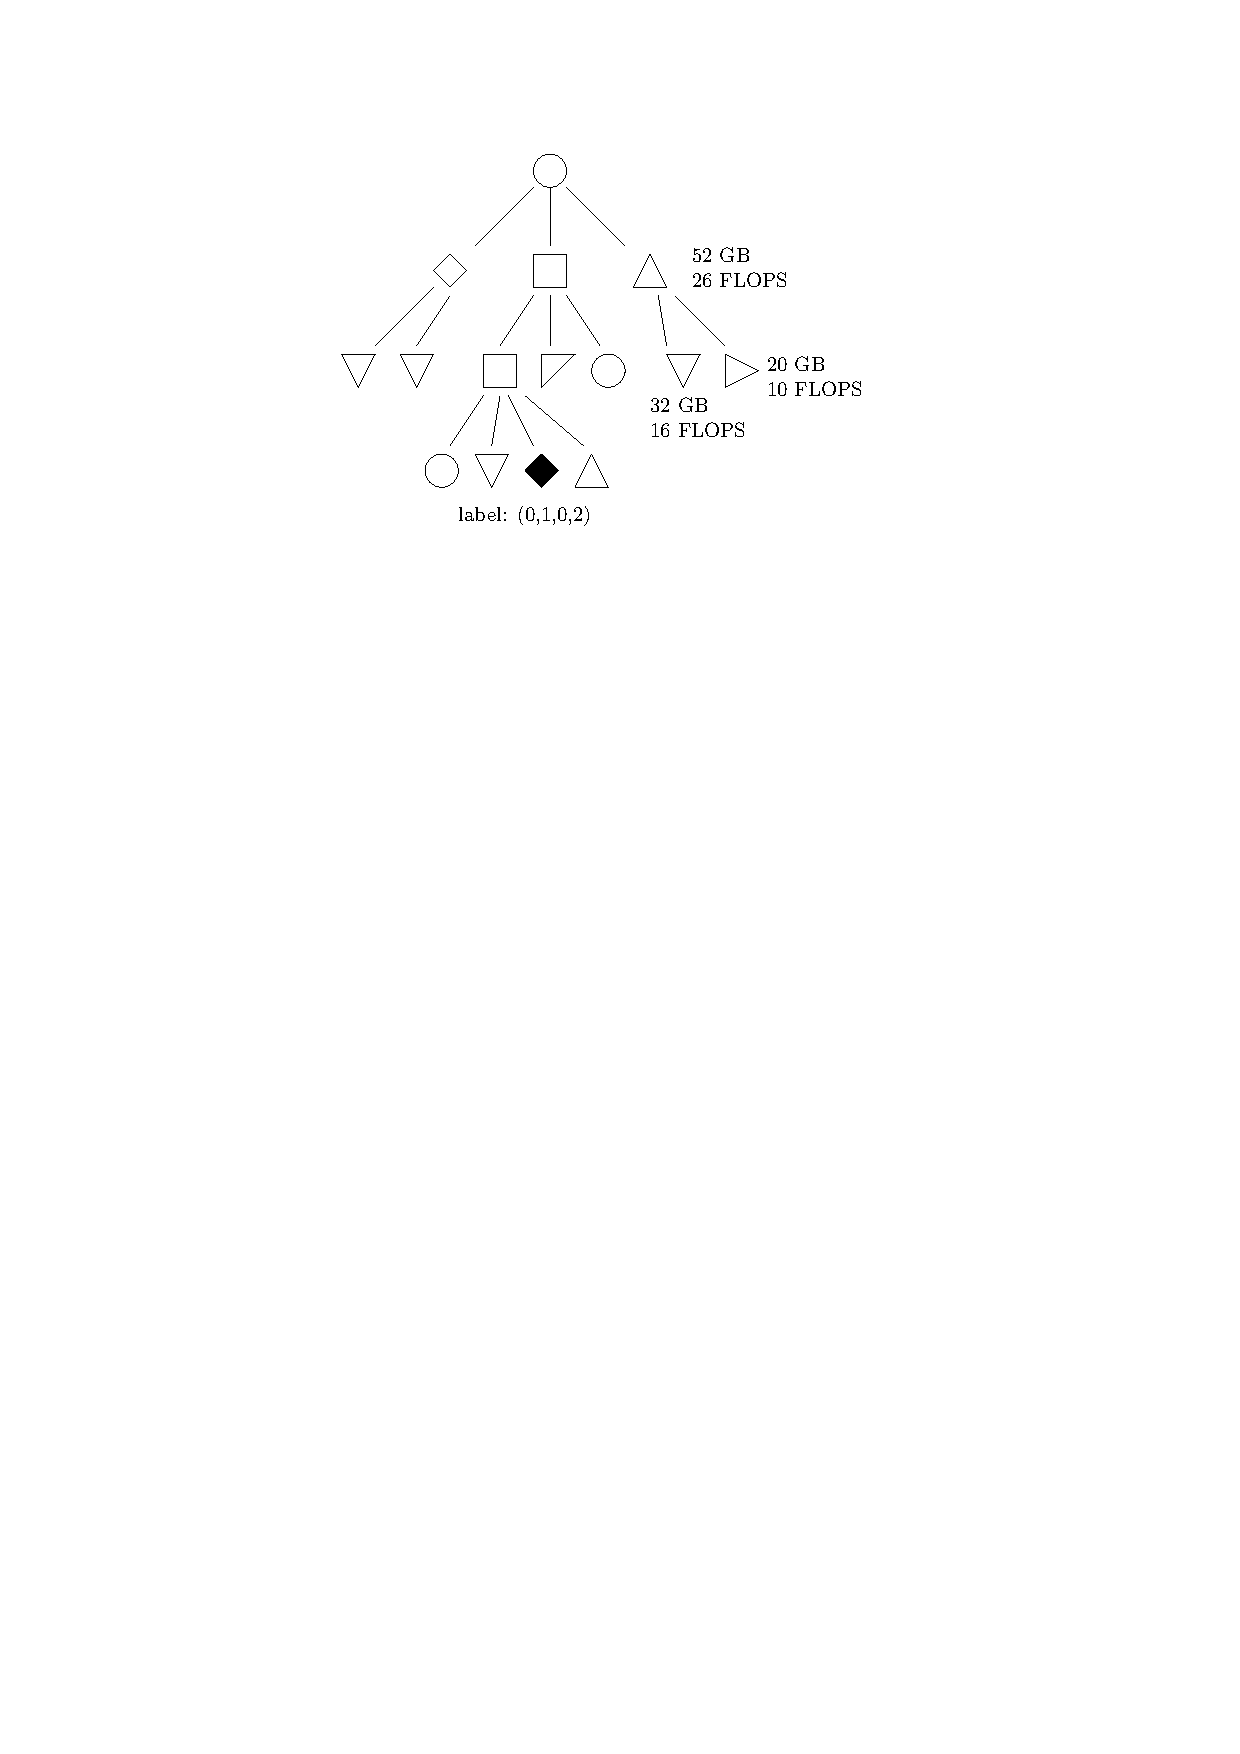
\includegraphics[scale=1]{heterog_tree}
	\caption{A heterogeneous physical network represented as a tree (same shapes do not indicate
	same nodes).}
	\label{fig:heterog_tree}
 \end{subfigure}	
 
 \begin{subfigure}{\textwidth}
    \centering
	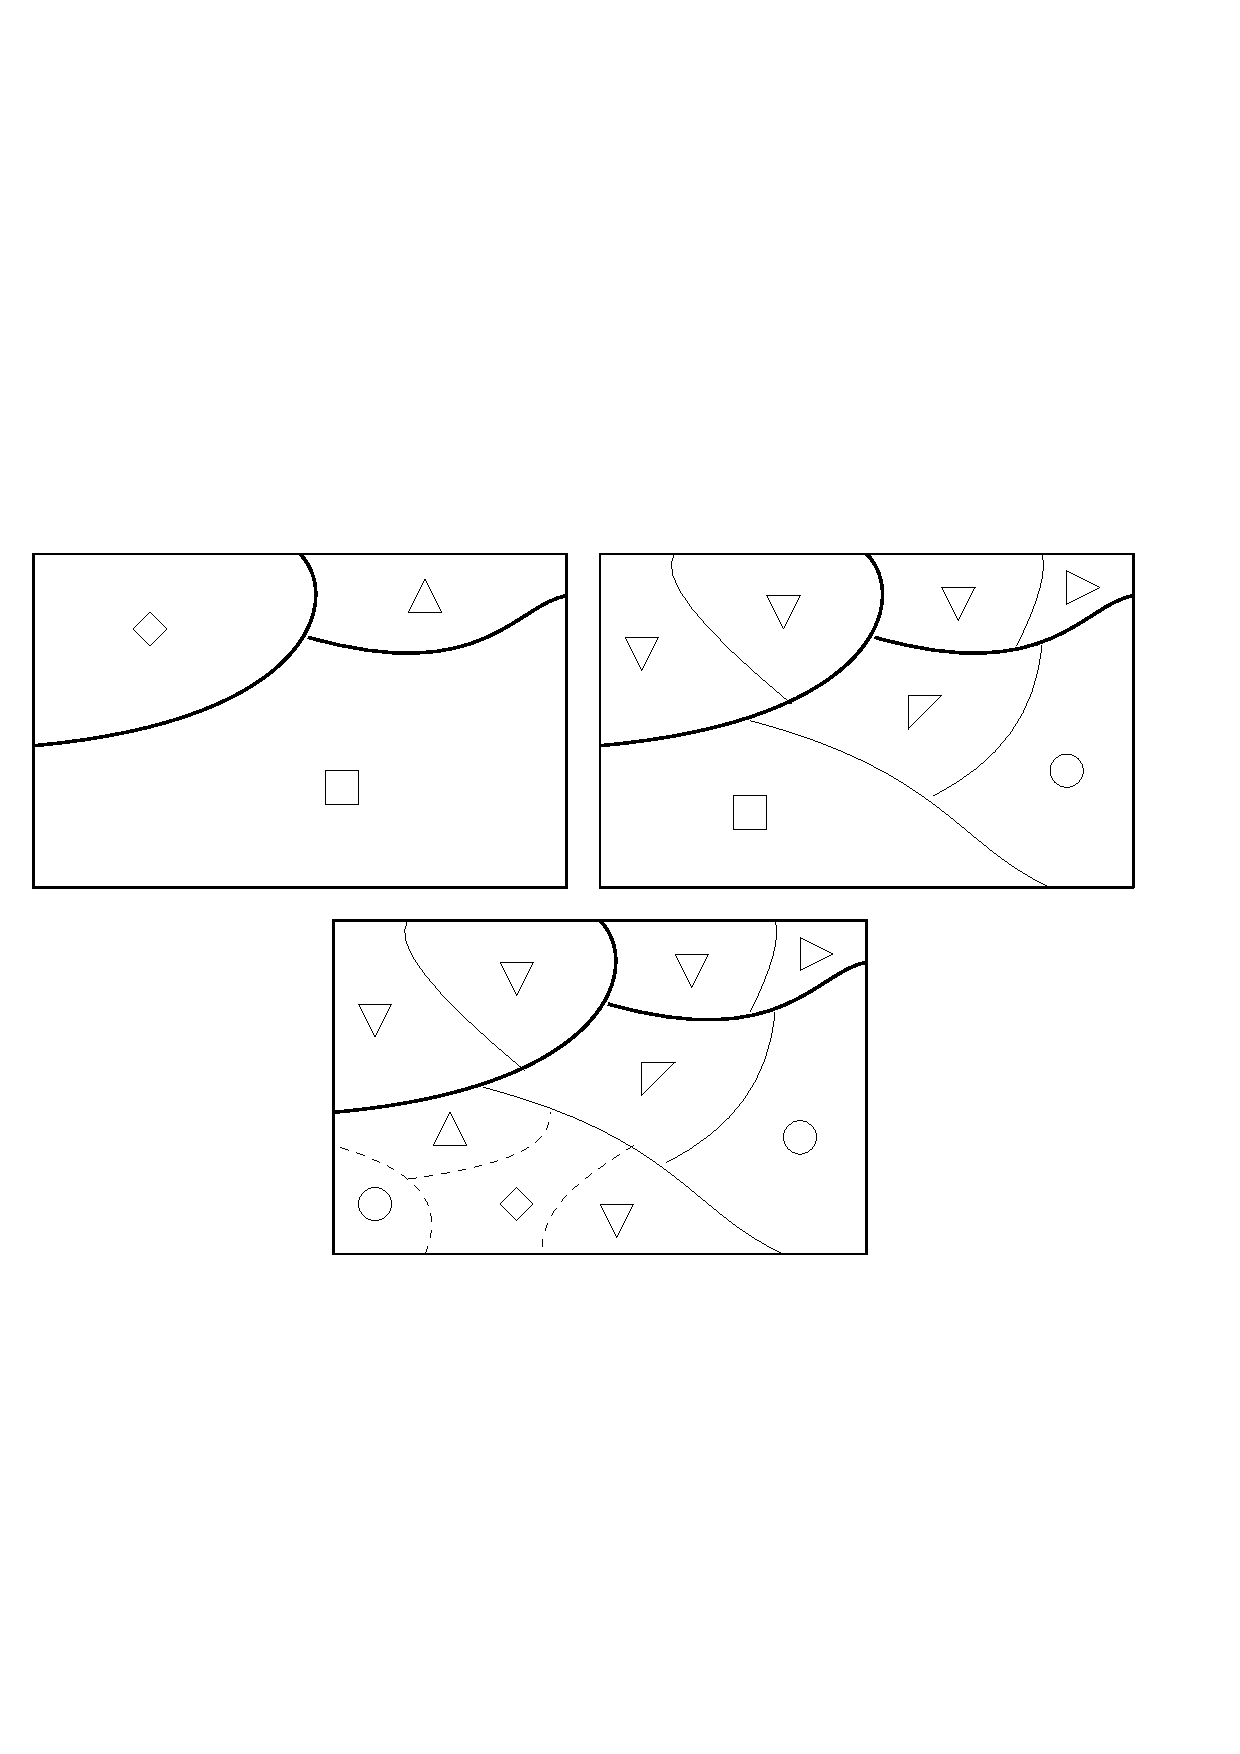
\includegraphics[scale=0.7]{heterog_tree_part}
	\caption{Recursively/hierarchically partioning the application according to the heterogeneous 
	tree. Every block has have different number of points/vertices and different weights.}
	\label{fig:heterog_part}
 \end{subfigure}
 \caption{ The physical network represented as a tree and a partition of the input mesh/graph 
 based on that.}
 \label{fig:heterog}
\end{figure}

\emph{Attention,} the local points should be traversed "as usual", meaning:
\begin{verbatim}
for( int i=0; i<localN; i++){
auto thisPoint = coords[i]; //this is not completely true...
...
}
\end{verbatim}

If done this way, the centers will be wrong. A center is the $x$-th element of a block. By $x$-th
we imply the order based on the sfc indices. Across PEs the points are distributed using the 
hilbert curve but within a PE, points are stored based in their index of the distribution.
For example, PE 2 will store points like $[10,13,20,25]$ where these numbers are their global
distribution indices, not the sfc indices. For that we must calculate the sfc index and sort 
the local points:
\begin{verbatim}
vector<> sfcIndices = getHilbertIndices( ... );
sort( sfcIndices );
for( int i=0; i<localN; i++){
//get the points by their order on the sfc
auto thisPoint = coords[ sfcIndices[i] ]; 
...                      ^^^^^^^^^^^^^
}
\end{verbatim}

\begin{algorithm}
//number of block for the already known partition\\
numOldBlocks = partition.max() \\
blockSizes( numOldBlocks ); \\
//calculate local size for each block\\
\For{all local points $i$}{
blockSizes[ partition[i] ]++;
}
\BlankLine

//get prefix sum\\
MPI\_send( blockSizes, root);\\
\If{ thisPE==root}{
calculate prefix sum for every block //see also \cref{fig:prefixSum}\\
}
//replicate prefix sum in every PE\\
MPI\_scatter( prefixSum );\\
\BlankLine

calculate global size for every block //something like prefixSum[b*p]\\
calculate center indices for every block // see \cref{eq:centers}\\
thisPE = comm$->$getRank);\\
\BlankLine

//sort indices based on their sfc index\\
sfcIndices = getHilbertIndices();\\
sort( sfcIndices );\\
\BlankLine

//and centersForBlock[b].size()=number of centers for block b
vector$<$vector$<$point$>$ centersForBlock( numOldBlocks );\\
\BlankLine

\For{int b=0; b$<$numOldBlocks; b++}{
//local range per block for this PE\\
from = b*(p+1)+thisPE;\\
rangeStart = prefixSum[ from ];\\
rangeEnd = prefixSum[ from+1 ];\\
//to calculate the within-block index of every point\\
counter = rangeStart;\\
  \For{ point c : center indices for this block}{
  	//center c is owned by thisPE\\
  	\If{ rangeStart$<$ c $<$rangeEnd}{
  	  \For{int i=0; i$<$localN; i++}{
		sortedIndex = sfcIndices[i];\\ 
		\If{sortedIndex==c}{
		  centersForBlock[b].push\_back( coords[sortedIndex] );
		}
		counter++;\\
  	  }
  	}
  }
}
//sum centers across all PEs\\
//deliberately on separate loop\\
\For{int b=0; b$<$numOldBlocks; b++}{
MPI\_sum(centersForBlock[b]);;
}
\caption{sketch code for findInitialCenters in hierarchical $k$-means}
\end{algorithm}



\subsection*{Assigning a block to every point}
\blue{Note that most of this section is more related to the multi-constraint \km\ version and less to
the hierarchical version}

In the homogeneous case, we calculate a global optimum size for all blocks. That is, find the total
node weight of the graph (every PE finds the local weight and we do a global sum). Then, the
optimum weight is globalWeight/k.

In the hierarchical version, the graph is already partitioned into numOldBlocks blocks. 
We are also given a CommTree level, i.e., a vector $L_h$ of CommTree nodes representing the current
hierarchy level $h$. Also, $L_h.size()$ is the total number of new blocks that we want to partition.
In order to get the number of new blocks per old block call CommTree::getGrouping($L_h$).
This returns a vector on how the nodes in $L_h$ are grouped. For example, in \Cref{fig:heterog}, 
level 2 has 7 nodes so $L_2.size()=7$ and call $A=$CommTree::getGrouping($L_2$).
Then, $A.size()=3$, $accumulate(A)=L_2.size()=7$ and $A=[2,3,2]$ indicating that the first 2 
nodes of $L_2$ have the same
father, i.e., belong to the same previous block. The same for the next 3 nodes and the last 2.
\\\todo{vector $A$ can also be returned (or converted) to a prefix sum of the sizes, similar to
array ia in the CSR matrix format. For $A$ in this example it would give $A=[0,2,5,7]$}

Every new block corresponds to an CommTree node, that is a group of PEs if the node is not a leaf
or a single PEs if the node is leaf. Leaf or not, every node has two properties: the memory capacity
and the computational speed of the PEs  it includes. Every new block must have at most as many
points as can fit in its memory and their total weight must be close to its speed. The memory
constraint is a \emph{hard} constraint and a PE cannot be overloaded with more points that it can fit. 
The speed is an \emph{soft} constraint; we can give points to a PE that require more
computational effort that it can offer but this will cause this PE to slow down the application.
Every block has also two properties: the number of points it contains and the sum of their weights.
PE memory corresponds to number of points per block and PE speed to block weight.
So the goal is to map blocks to PEs by always respect the memory constraint of the PEs but also
minimize the difference between PE speed and block computational weight.

Let $f$ be a mapping from a block $b$ to a PE $p$, then
\begin{align*}
\forall \;block\;b,\; & b.numPoints \leq f(b).memory \\
& b.weight \leq (1+\epsilon)f(b).speed \\
& or\\
& (1-\epsilon)f(b).speed \leq b.weight \leq (1+\epsilon)f(b).speed \\
\end{align*}

This means that in the 2-constraint \km\ there are 2 imbalances that need to be calculated per block
while before it was only one. In the more general case, we have to maintain as many imbalances
as the number of constraints. In the non-hierarchical version, (the one) imbalance was
calculated as
\begin{align*}
& optSize = totalWeightSum/k \\
&imbalance = (maxBlockWeight-optSize)/optSize
\end{align*}
and did not considered block weights. This must be changes so to consider two imbalances:
block weights and block number of points.
\\\todo{? should we keep an imbalance per old block or just one (or two here) global imbalance?}


\subsection*{Sort centers by distance to the bounding box of the PE}

To optimize how we check the centers for every point, we can sort according to their distance
from the bounding box of every PE.

\begin{figure}
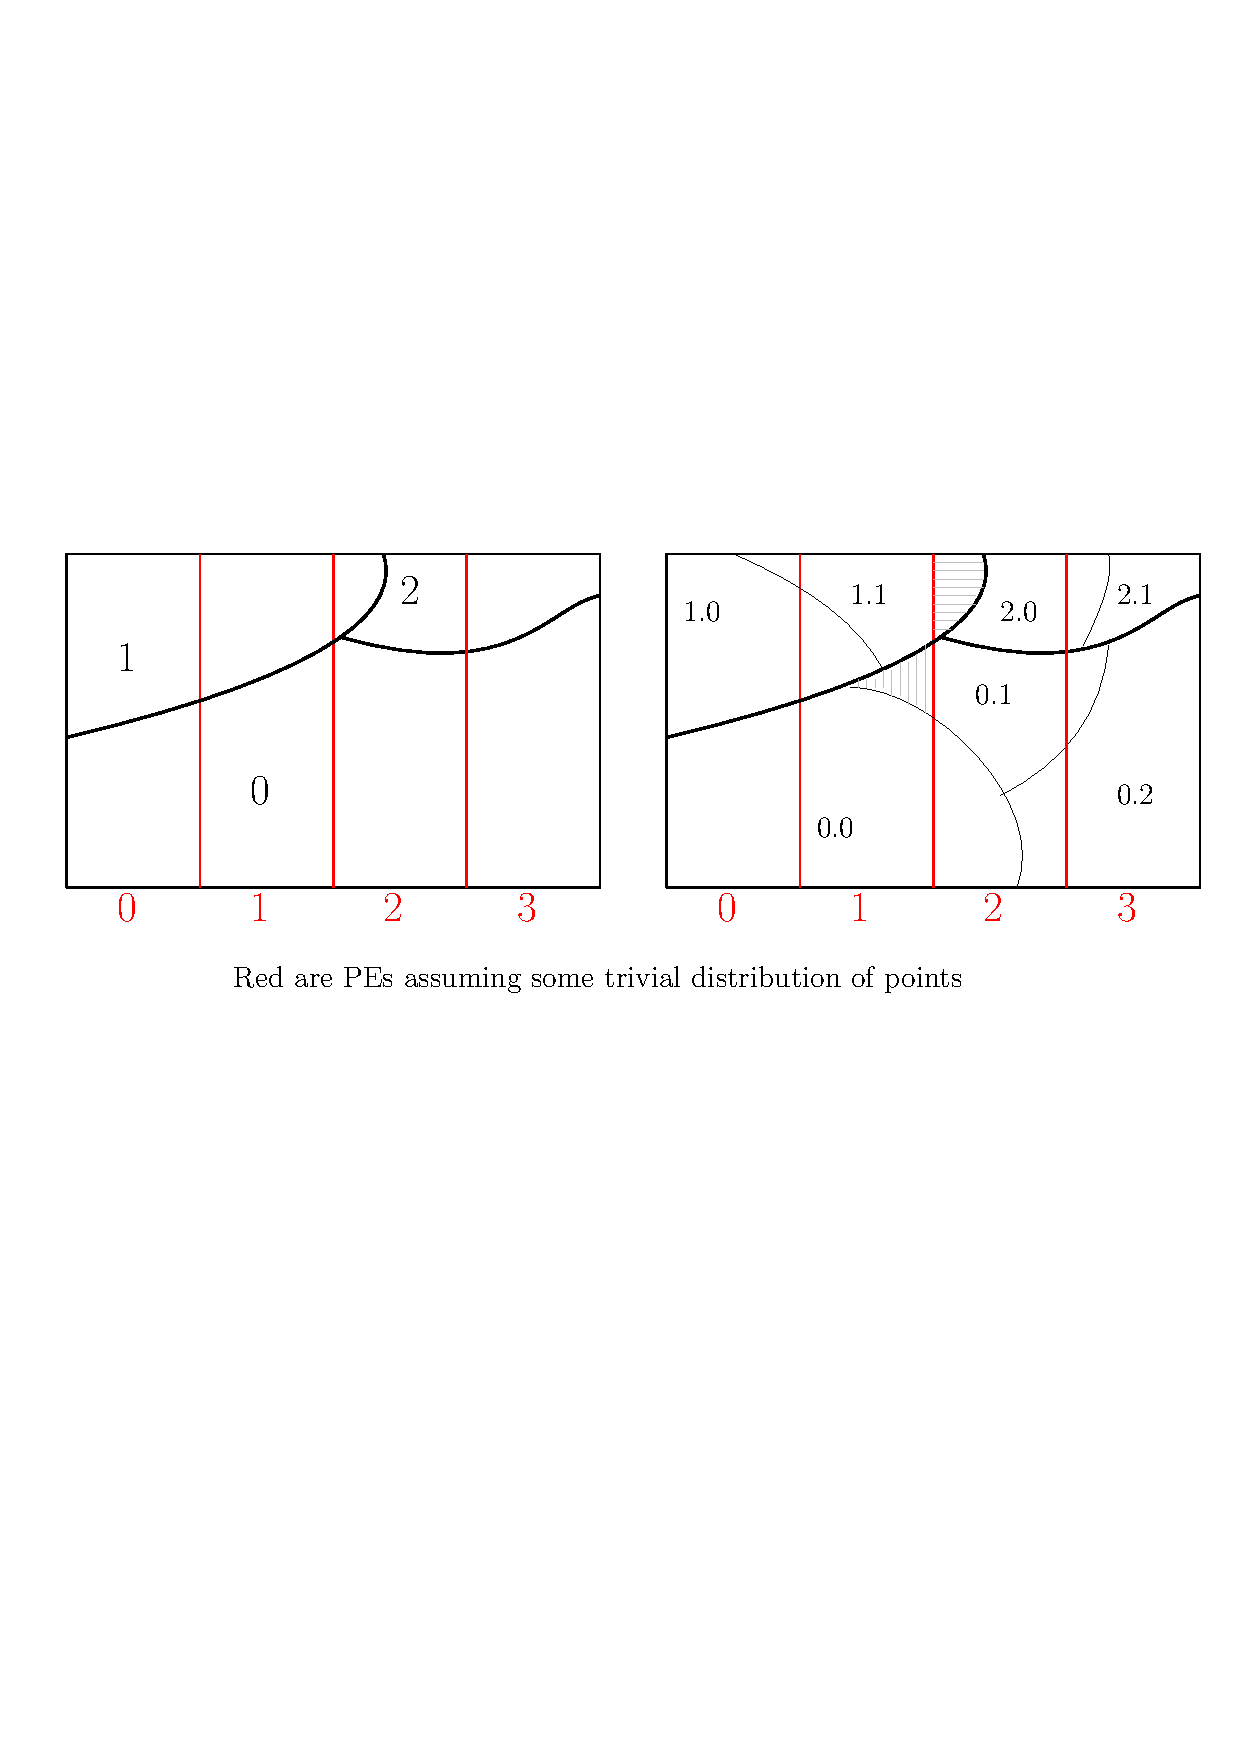
\includegraphics[scale=0.7]{heterog_tree_part_with_PEs}
\caption{With red is the distribution of points into PEs and with black the known partition.
Here we have 4 PEs and the mesh is partitioned first in 3 parts and then in 3,2 and 2 respectively.}
\label{fig:heterog_withPEs}
\end{figure}


\subsection*{Repartition with hierarchical k-means}

The current code (03 May 2019) of the hierarchical k-means accepts as one of the inputs the centers.
The centers are of type \texttt{vector<vector<point>> centers} and the centers.size() implies
the number of parts in the previous hierarchy level. In general, the algorithm will receive
a partitioned mesh, say into $k$ parts, and will partition it again into $k'$ parts with $k'>k$.
For example, we all ready have 3 parts ($k=3$) and each part will be partitioned into 5 parts
giving in total 15 parts ($k'=15$). 

In repartition, we want a mesh that is already partitioned into $k$ parts to be repartitioned in $k$
parts (there are other scenarios but this is the most usual one). With the code as it is, this is not
possible. 

Started (03/05) adapting the code in k-means to handle some input parameters differently when we
want to repartition. I am afraid this cannot be avoided...



\end{document}
